%   Copyright 2016 Emilio Rojas
%
%   Licensed under the Apache License, Version 2.0 (the "License");
%   you may not use this file except in compliance with the License.
%   You may obtain a copy of the License at
%
%       http://www.apache.org/licenses/LICENSE-2.0
%
%   Unless required by applicable law or agreed to in writing, software
%   distributed under the License is distributed on an "AS IS" BASIS,
%   WITHOUT WARRANTIES OR CONDITIONS OF ANY KIND, either express or implied.
%   See the License for the specific language governing permissions and
%   limitations under the License.

La simulación del problema se ha hecho en la versión 9.2.30.221 del software
TINA de DesignSoft.

\bigskip

\usubsection{Circuito}

En general el circuito es el mismo del problema. En las notas se especifican las
diferencias existentes entre el circuito del problema y el planteado.
\begin{center}
  \begin{figure}[H]
    \centering
    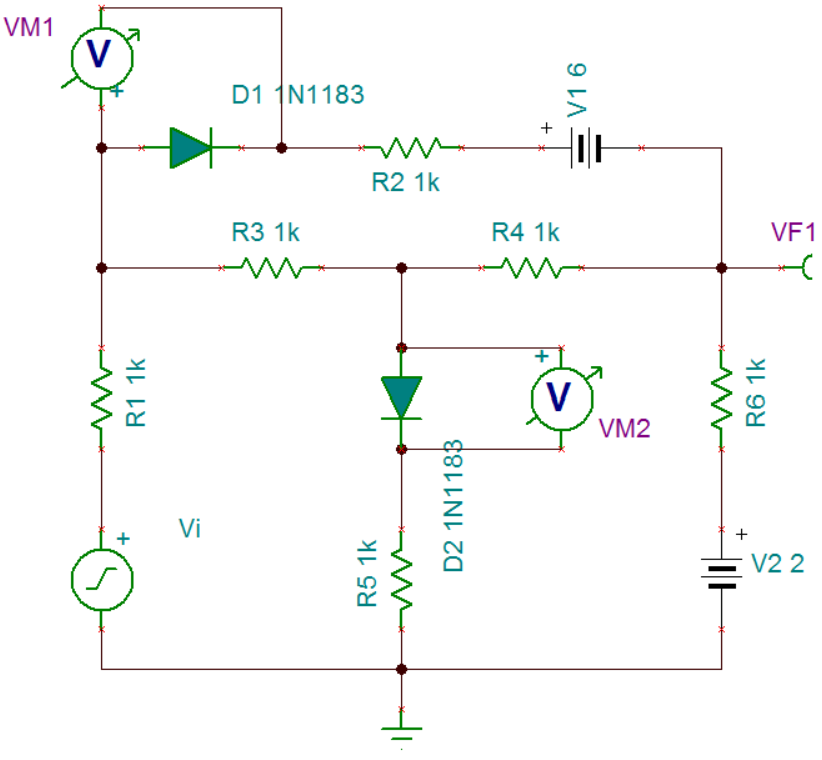
\includegraphics
    [width=0.5\textwidth]
    {simulacion/circuito-tina.png}
    \caption{Circuito simulado.}
  \end{figure}
\end{center}

\usubsection{Metodología}

Se ha realizado un análisis del estado transitorio para un período y medio, esto
con el fin de no ser redundante pero a la vez presentar de manera clara los
cambios en los estados de los diodos.

Para realizar el análisis se accedió a la opción
\texttt{Analysis>Transient...} del menu principal de TINA.

\begin{center}
  \begin{figure}[H]
    \centering
    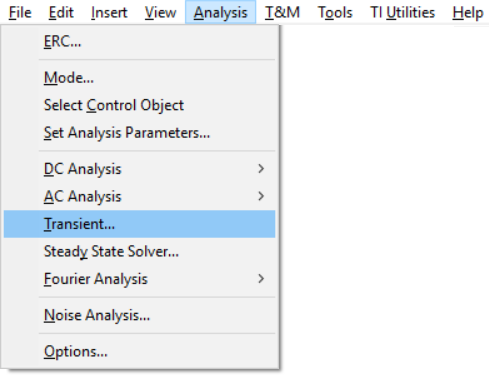
\includegraphics
    [width=0.5\textwidth]
    {simulacion/menu-analisis.png}
    \caption{Opción utilizada.}
  \end{figure}
\end{center}

Para mostrar el período y medio mencionado, deben ajustarse los tiempos de
inicio y fin del gráfico a generar, se han ajustado a 0 segundos en el caso del
inicio, y 30 miliSegundos en el caso del final. La diferencia de estos valores
está relacionada con la frecuencia de la fuente, y puede ser ajustada para
visualizar una mayor o menor franja de tiempo.

\begin{center}
  \begin{figure}[H]
    \centering
    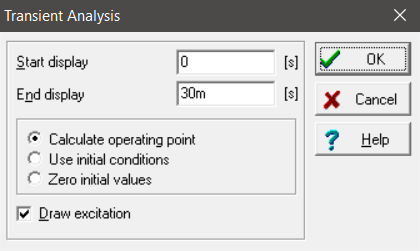
\includegraphics
    [width=0.4\textwidth]
    {simulacion/analisis-opciones.png}
    \caption{Ajustes del análisis.}
  \end{figure}
\end{center}

\newpage
El gráfico que se obtiene es el siguiente:

\begin{center}
  \begin{figure}[H]
    \centering
    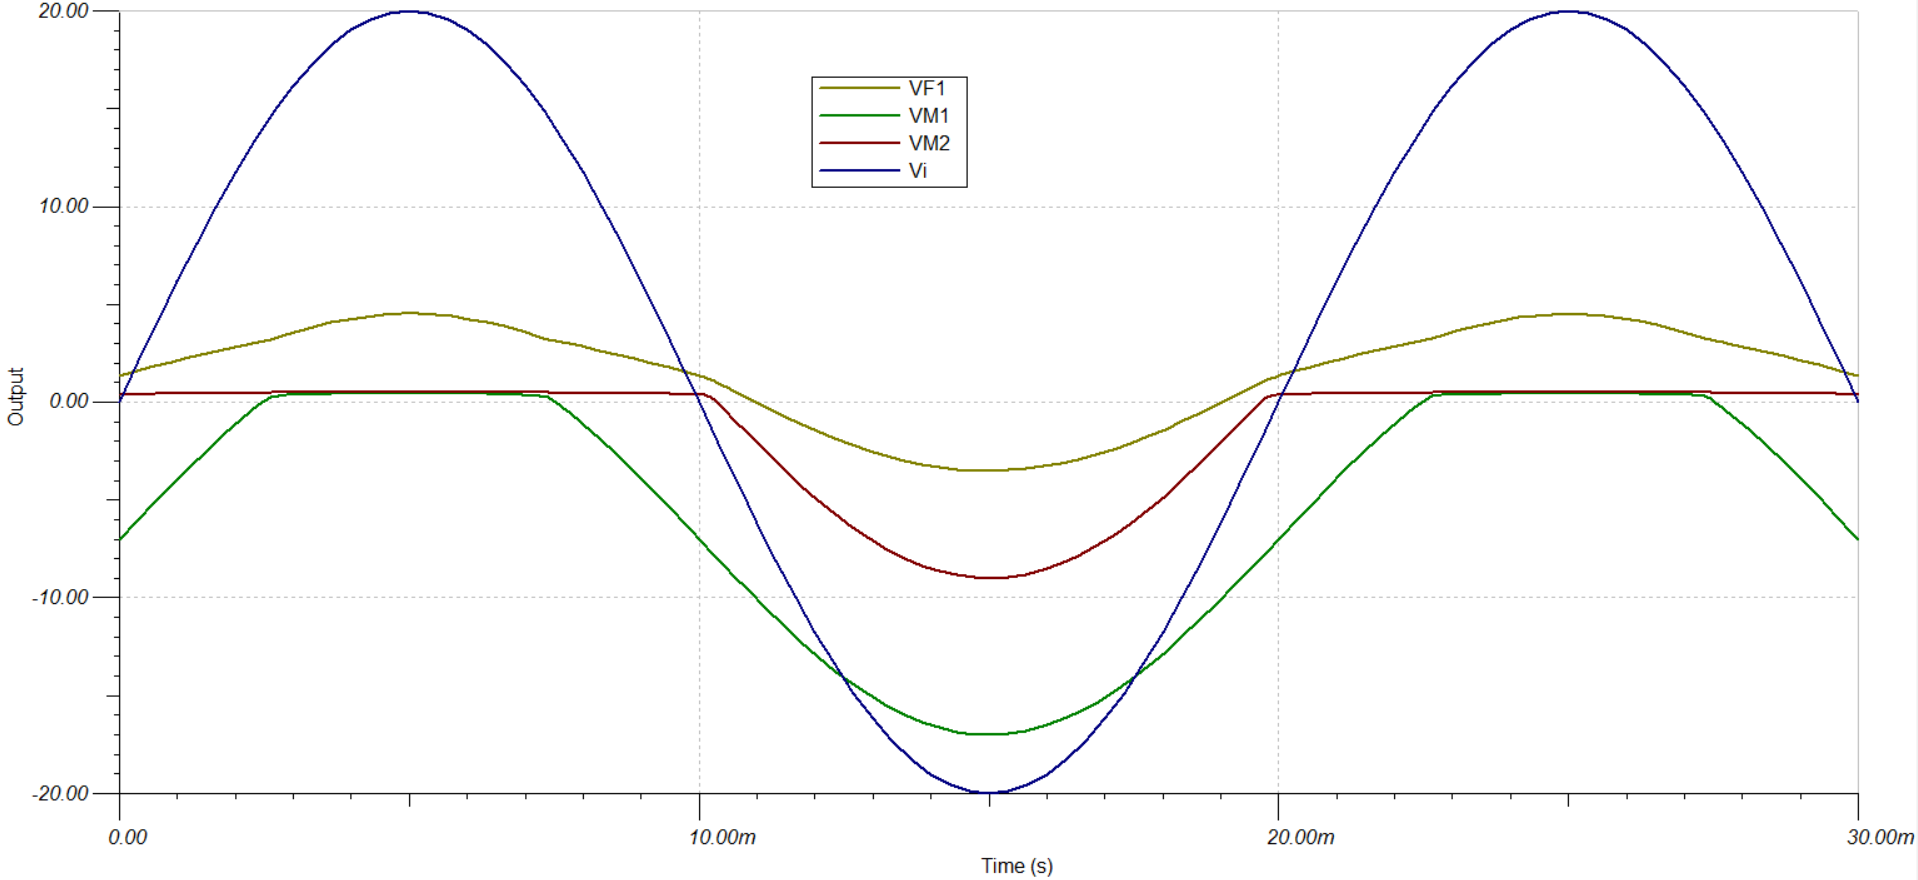
\includegraphics
    [width=\textwidth]
    {simulacion/analisis-grafico.png}
    \caption{Gráfico obtenido.}
  \end{figure}
\end{center}

Debe tomarse en consideración que VF1 corresponde a $V_o$, VM1 y VM2
corresponden a los voltímetros 1 y 2, que a su vez corresponde a los diodos
$D1$ y $D2$ respectivamente.

\usubsection{Observaciones}
Analizando los diodos en un comportamiento ideal, tomando $D1$ off, $D2$ off, se
obtuvo que esto ocurre cuando el valor del voltaje de entrada es menor o igual
a -2V, y los valores del voltaje de salida van entre 1.5V y -4V aproximadamente.
Esto se obtiene del análisis de la figura 1.
En la figura 2, se observa que el diodo $D1$ estará off y $D2$ estará ON, cuando
el voltaje de entrada sea mayor a -2V y menor o igual a 14V. Los valores del
voltaje de salida irán desde 1.5V a 2.5V, aproximadamente.

Los dos diodos conducirán, cuando el valor del voltaje de entrada sobrepase los
14V. Los valores del voltaje de salida tendrán valores próximos entre los 2.5V
a los 4.5V.

En la figura 5, se toman todos los comportamientos de los diodos y se saca la
gráfica del comportamiento del circuito según la polarización de cada diodo.
Esta figura es comparada con la figura 9, la cual es la grafica obtenida del
análisis en simulación y se observan datos muy parecidos, pero con ciertas
variaciones en los voltajes de salida, lo cual es normal por las variaciones en
un análisis experimental. Si bien leve la diferencia, los diodos en su estado on
durante la simulación no permanecen en 0V, sino que un poco más, igualmente el
cambio de estado on a off no es instantaneo, sino gradual. Es apreciable de la
figura 9 la razón por la cuál el caso en que el diodo $D1$ esté on y el $D2$ off
no se da, puesto que no coinciden las gráficas para que suceda el caso,
contrario al caso en que $D1$ está off y $D2$ está on.

En general se puede decir que las diferencias son mínimas entre el gráfico del
modelo ideal y de la simulación. Si no se precisa una exactitud estas
diferencias pueden ser despreciadas y considerar los gráficos de la figura
5 y la 9 iguales.

\bigskip

\textbf{Notas}
\begin{itemize}
  \item La simulación se ha hecho con diodos reales(no ideales) 1N1183 provistos
  por el software. Pese a que se ha investigado sobre la posibilidad de utilizar
  diodos ideales en TINA, no se ha encontrado mayor información al respecto(se
  nota que es posible cambiar los parámetros de los diodos), y no se ha aplicado
  lo encontrado. Esto da cabida a la comparación de los gráficos obtenidos según
  los resultados contra los simulados.
  \item Se han utilizado voltímetros en los diodos para corroborar el estado de
  estos contra los valores obtenidos en la solución. Los voltímetros no afectan
  el circuito del problema.
  \item Ante la necesidad de utilizar una frecuencia para la fuente sinusoidal,
  se ha utilizado $f = 50Hz$, que es la predeterminada del software.
  \item El circuito utiliza una tierra para referenciar a $V_o$.
\end{itemize}
